\chapter{文件系统、写回与崩溃一致性}

\begin{keyidea}
“write 返回”只说明某层接受了数据，不自动等于磁盘已经持久。显式盘面编码、
块树、缓存状态、IRQ14 请求、ATA FLUSH、ordered journal、commit、
checkpoint 与 replay 共同建立跨重启仍可证明的顺序。
\end{keyidea}

\section{从扇区到可命名持久对象}

管道中的字节在最后一个持有者退出后消失；磁盘中的字节则要跨越进程结束、
内核停止乃至整机重启继续存在。两者都可以提供 \code{read/write}，但生命
周期完全不同。文件系统的核心工作不是“把数组写进磁盘”，而是同时回答：

\begin{enumerate}[label=\arabic*.]
  \item 哪些扇区属于启动链，哪些扇区属于文件系统；
  \item 哪些块空闲，哪些块由哪个 inode 拥有；
  \item 名称如何逐级解析到稳定 inode；
  \item 多个元数据块只写完一部分时，下次启动怎样识别；
  \item 用户指针、文件描述符、缓存和设备完成之间如何划界。
\end{enumerate}

早期磁盘操作系统常把连续扇区直接分给文件。文件增长后，连续空洞越来越难找，
于是出现链式分配、索引分配和 inode。Multics 与 UNIX 又把目录层次、权限和
设备抽象放到同一命名空间中。现代 ext4、XFS、ZFS 已包含日志、extent、
校验、延迟分配和复杂恢复；直接移植其中任何一个都会隐藏本阶段最重要的状态
转换。v0.11 因此采用固定布局和十个直接块，把范围压小到可以逐字节审计。

\begin{contractbox}
本阶段的完成定义不是“同一次运行可以读回刚写的数据”。磁盘必须在关闭 QEMU
后保留内容，第二个全新来宾实例必须先读到旧内容；超级块被宿主故意破坏后，
第三个实例必须拒绝挂载且不能用自动格式化掩盖故障。
\end{contractbox}

\topic{磁盘分区边界先于文件系统格式}
启动磁盘精确为 2 MiB，即 4096 个 512 字节扇区。LBA 是扇区编号，不是字节
地址；字节偏移由
\[
  \mathrm{offset}=\mathrm{LBA}\times512
\]
得到。当前边界为：

\begin{osgridlongtable}{L{0.19\textwidth}L{0.27\textwidth}L{0.42\textwidth}}
LBA 半开区间 & 所有者 & 不变量\\ \hline
\endfirsthead
LBA 半开区间 & 所有者 & 不变量\\ \hline
\endhead
\code{[0,2048)} & 固件描述符、Stage 1、Kernel 描述符与 ELF &
打包器证明 Kernel 负载结束位置不越过 2048\\ \hline
\code{[2048,3072)} & v0.11 文件系统 & 1024 个固定大小逻辑块\\ \hline
\code{[3072,4096)} & 保留 & 当前必须不被文件系统分配\\ \hline
\end{osgridlongtable}

最初设计把文件系统放在 LBA 1024。宿主内存块测试全部通过，但真实 Kernel
ELF 增长到 505 KiB 后，其 LBA 66 起的负载已经延伸到约 LBA 1054。QEMU
第一次挂载看到的“超级块”其实是 Kernel ELF 尾部，正确地报告 CRC 或 magic
损坏。这个失败说明布局必须由最终产物验证，不能由设计时估计保证。

修正不是把文件系统起点挪到“当前内核尾部再加一点”，而是建立稳定的 1 MiB
边界。Python 打包器现在拒绝任何跨过 LBA 2048 的 Kernel 负载，C++
格式常量从同一边界开始。内存块设备扩大到 4096 扇区，使宿主模型和目标磁盘
具有相同地址上界。

\begin{keyidea}
磁盘布局是跨启动阶段的 ABI。只修改内核常量而不修改镜像生成器、审计器、
测试设备和教材，会制造多个互相矛盾的“真相”。
\end{keyidea}

\topic{ATA PIO 写入是一条可失败的硬件状态机}
v0.7 的读取路径已经会选择 primary master、写 LBA28 寄存器、发
\code{READ SECTORS} 命令并等待 DRQ。写入不能简单把 \code{inw} 换成
\code{outw}；命令、数据方向和持久化完成具有不同阶段。

\begin{enumerate}[label=\arabic*.]
  \item 向设备控制端口写入禁用设备中断位，使当前轮询状态机独占完成事件；
  \item 轮询状态端口，等待 BSY 清零，同时拒绝 ERR 与 DF；
  \item 写 drive/head、扇区数 1、LBA low/mid/high；
  \item 向命令端口写 \code{WRITE SECTORS} 的 \code{0x30}；
  \item 等待 DRQ，证明设备已经准备接收一个扇区；
  \item 把 512 字节按小端组合成 256 个 \code{uint16_t}，逐字写数据端口；
  \item 等待 BSY 再次清零，拒绝设备错误；
  \item 事务屏障处发送 \code{FLUSH CACHE} 的 \code{0xE7} 并等待完成。
\end{enumerate}

\begin{pdfdiagram}
  \node[os state] (idle) {非忙};
  \node[os block,right=of idle] (command) {写 LBA\\发 0x30};
  \node[os hardware,right=of command] (drq) {DRQ=1};
  \node[os block,below=of drq] (data) {256 次 outw};
  \node[os state,left=of data] (complete) {BSY=0};
  \node[os hardware,left=of complete] (flush) {0xE7 flush};
  \draw[os arrow] (idle) -- (command);
  \draw[os arrow] (command) -- (drq);
  \draw[os arrow] (drq) -- (data);
  \draw[os arrow] (data) -- (complete);
  \draw[os arrow] (complete) -- (flush);
\end{pdfdiagram}
\diagramnote{DRQ 只说明可以传输数据；BSY 清零只说明命令结束；事务需要的持久化边界由显式 flush 提供。}

每个轮询都有固定预算。永久忙返回 \code{BusyTimeout}，一直没有 DRQ 返回
\code{DataRequestTimeout}，ERR/DF 返回 \code{DeviceError}。文件系统不
依赖具体 ATA 错误枚举，只通过 \code{FileSystemBlockDeviceStatus} 接收
读、写、flush 成败。宿主测试以同一接口挂接内存设备，目标内核挂接
\code{AtaPioDevice}。

\topic{磁盘格式只由显式字节编码定义}
C++ 结构体适合内存中的类型检查，不适合直接成为持久格式。编译器可能插入
padding，枚举宽度和对齐规则也属于 ABI。v0.11 对每个多字节字段显式执行
little-endian store/load；磁盘格式由偏移表定义。

\topic{超级块}
相对块 0 是 512 字节超级块。前 8 字节为 \code{OSFSV001}，随后以
\code{uint64_t} 保存版本、块大小、总块数、inode 位图、inode 表、数据
位图、数据区、数量、根 inode、事务状态和代次。偏移 508 保存对前 508
字节计算的 IEEE CRC32。

\begin{osgridlongtable}{L{0.17\textwidth}L{0.18\textwidth}L{0.53\textwidth}}
相对块 & 数量 & 内容\\ \hline
0 & 1 & superblock、事务状态与 CRC32\\ \hline
1 & 1 & 32 位有效范围的 inode bitmap\\ \hline
2--9 & 8 & 32 个固定 128 字节 inode\\ \hline
10 & 1 & 1013 位有效范围的数据块 bitmap\\ \hline
11--1023 & 1013 & 目录项和普通文件数据\\ \hline
\end{osgridlongtable}

bitmap 仍占完整扇区，但有效位之外必须全零。这个规则能发现错误循环把位图
扫描到 4096 位、或未来格式被旧内核误读的情况。inode 0 永久保留，inode 1
固定为根目录。

\topic{inode}
每个 inode 精确 128 字节：类型、文件长度、代次、链接数、已分配块数、
十个 64 位相对块号、四字节保留区和 CRC32。普通文件与目录都最多使用十个
直接块，因此显式上限为
\[
  10\times512=5120\ \text{bytes}.
\]
使用 \code{uint64_t} 保存块号和长度是为了让内存接口以后扩展时不必整体
改型；这不取消当前格式的语义上限。

直接块不是 ATA 绝对 LBA，而是文件系统区域内的相对块。I/O 前统一加
\code{OS_KERNEL_FILE_SYSTEM_START_LBA}，避免把格式绑死到物理分区位置。

\topic{目录项}
目录内容由连续的 64 字节目录项组成。每项包含 64 位 inode 号、64 位类型、
64 位名称长度和 40 字节名称。名称不是以 NUL 结尾；长度是唯一边界，剩余
字节编码时清零。当前拒绝空名称、超过 40 字节、斜杠、C0 控制字符、
\code{DEL}、\code{.} 和 \code{..}。

目录本身也是 inode，其 \code{size_bytes} 必须是 64 的整数倍。一个块容纳
8 项，十个直接块最多容纳 80 项。inode 不保存路径；路径来自从根目录开始
的一串目录项，这正是 rename 不需要搬动文件数据的原因。

\topic{CRC 能发现变化，但不能证明所有权正确}
CRC32 对随机位翻转很敏感，适合发现镜像损坏、偏移错误和部分写入。它不是
密码学认证，也不能发现“字段本身合法但引用了错误对象”的语义损坏。例如两个
inode 各自 CRC 都正确，却可能引用同一数据块；目录项也可能引用未分配 inode。

挂载因此分两层：

\begin{enumerate}[label=\arabic*.]
  \item 解码层检查 magic、版本、布局、枚举、长度、CRC 和保留范围；
  \item 一致性层联合检查 bitmap、inode、目录项、块唯一性和根可达性。
\end{enumerate}

只有超级块整扇区全零时才允许格式化。非零但 magic 或 CRC 错误说明磁盘曾有
内容或边界错误，必须返回 \code{Corrupt}。如果此时自动格式化，恰好会把最
重要的故障证据覆盖掉。

\topic{bitmap 分配把空间所有权变成守恒关系}
inode 分配从编号 2 开始寻找第一个零位；数据块分配在 1013 个有效位中寻找
零位，再转换为相对块 \code{11+bit_index}。释放文件时逐个验证块位于数据区，
清对应位，并把 inode 的直接块、块数和长度归零。

一致性检查维护一张 \code{seen_data_bitmap}。遍历每个已分配 inode 时：

\begin{itemize}
  \item 前 \code{allocated_block_count} 个直接块必须位于数据区且 bitmap 为 1；
  \item 同一块在 \code{seen_data_bitmap} 中不能已经出现；
  \item 块数之后的直接块必须为零；
  \item 最终 data bitmap 的每个有效位必须与 seen 位完全相等。
\end{itemize}

所以“位图说已分配但没有 inode 拥有”和“inode 使用了位图中的空闲块”都会
失败。文件所需块数还必须等于
\[
  \left\lceil\frac{\mathrm{size_bytes}}{512}\right\rceil,
\]
不接受隐藏的尾部已分配块。

\topic{八项写回缓存具有明确状态转换}
块缓存固定八项，每项保存 512 字节、绝对 LBA、valid、dirty 和单调访问
代次。读取命中只复制缓存；未命中选择无效项或最小代次项。若淘汰项为 dirty，
必须先写回设备。写接口接收完整块，因此未命中时不必先读旧扇区。

\begin{pdfdiagram}
  \node[os state] (invalid) {invalid};
  \node[os block,right=of invalid] (clean) {valid clean};
  \node[os state,right=of clean] (dirty) {valid dirty};
  \draw[os arrow] (invalid) -- node[above]{read fill} (clean);
  \draw[os arrow] (invalid) to[bend right] node[below]{full write} (dirty);
  \draw[os arrow] (clean) -- node[above]{write} (dirty);
  \draw[os arrow] (dirty) to[bend left] node[below]{flush} (clean);
  \draw[os arrow] (clean) to[bend left] node[above]{evict} (invalid);
\end{pdfdiagram}
\diagramnote{缓存命中是性能状态；dirty 是持久化状态。两者不能用同一个布尔含义替代。}

\code{Sync} 逐项写回 dirty 块，再调用设备 flush。统计命中、未命中、淘汰、
设备读写和 flush 次数，但热路径不打印逐块日志；内核只在挂载、同步和最终
一致性检查处输出汇总。

\topic{Dirty/Clean 协议先保证可检测，再讨论恢复}
创建目录、创建/截断文件和写文件会同时改变多个块。v0.11 使用超级块中的
\code{transaction_state} 和 64 位代次建立最小提交协议：

\begin{enumerate}[label=\arabic*.]
  \item 完成路径、权限和容量预检；
  \item 代次加一，把超级块写为 Dirty，flush；
  \item 修改 bitmap、inode、目录项和数据缓存；
  \item \code{BlockCache::Sync} 写回全部 dirty 块并 flush；
  \item 把超级块写为 Clean、重算 CRC，再 flush。
\end{enumerate}

\begin{osgridlongtable}{L{0.21\textwidth}L{0.28\textwidth}L{0.39\textwidth}}
停止位置 & 磁盘可见状态 & 下次挂载\\ \hline
步骤 1 以前 & 上一份 Clean 格式 & 正常挂载\\ \hline
步骤 2--4 & Dirty，元数据可能部分新旧混合 & 报未完成事务并停止\\ \hline
步骤 5 完成 & 新一代 Clean 格式 & 正常挂载\\ \hline
\end{osgridlongtable}

容量不足属于正常业务结果，不应故意留下 Dirty。实现因此在写 Dirty 前统计
空闲 inode/数据块和目录容量。真正设备失败发生后则不能假装回滚成功：
超级块保持 Dirty，当前实例进入失败状态。

这不是日志。它保证“检测并停止”，不保证自动恢复。下一阶段可在独立日志区
保存 redo 记录和 commit record，再根据代次重放；只有到那时 Dirty 才能
进入恢复状态机。

\topic{路径解析从根目录逐组件证明类型}
当前只接受绝对路径，最长 128 字节。解析器先验证第一个字节是 \code{/}，
再扫描每个组件；不使用 NUL 终止，也不访问路径长度之外的用户内存。
\code{/} 直接得到根 inode，其他路径按以下循环：

\begin{enumerate}[label=\arabic*.]
  \item 当前 inode 必须是目录；
  \item 按 64 字节步长扫描目录项；
  \item 比较名称长度，再比较精确字节；
  \item 目录项引用必须在 inode bitmap 中已分配；
  \item 读目标 inode，并证明类型与目录项冗余类型一致。
\end{enumerate}

创建 \code{/shared/payload.bin} 时先解析父路径 \code{/shared}，证明最后
组件尚不存在，再分配 inode 并向父目录尾部追加目录项。目录需要新数据块时，
先分配并清零完整块，防止旧释放内容被解释为目录项。

\topic{根可达性检查拒绝孤儿、环和重复引用}
只遍历 inode bitmap 会接受孤儿 inode：它有合法 CRC 和数据块，但没有任何
路径可以到达。v0.11 在完成局部校验后，以 inode 1 为起点执行最多 32 项的
有界广度优先遍历。

\begin{enumerate}[label=\arabic*.]
  \item 把根 inode 放入固定队列和 reachable bitmap；
  \item 取出目录，解码每个目录项；
  \item 若目标已 reachable，则当前无硬链接格式下视为重复引用或环；
  \item 否则标记并入队；
  \item 遍历结束后逐位比较 reachable bitmap 与 inode bitmap。
\end{enumerate}

队列容量等于 inode 总数，所以不需要堆。根以外每个已分配 inode 必须恰有
一条来自可达目录的引用，当前链接数必须为 1。宿主集成测试直接翻转 inode
位图中的空闲位，证明孤儿被拒绝；另一项把根目录名称字节从 \code{s} 改为
\code{DEL}，证明格式正确但语义非法的目录项也被拒绝。

\topic{文件描述符把用户整数绑定到每进程句柄}
每个 PCB 有四个 \code{FileSystemHandle} 槽。用户看到的 fd 只是槽索引，
句柄保存 inode 号、当前偏移、读写能力和 open 状态。分别打开同一文件得到
独立偏移；本阶段没有 \code{dup}，因此尚无共享 open-file-description。
进程退出或用户异常时，运行时在销毁地址空间前关闭全部仍开放的槽。

\code{INT 0x80} 新增编号 10--15：Open、Read、Write、Close、Mkdir 和
Sync。第三参数使用 RDX。用户包装器按 System V ABI 收到
\code{RDI=number, RSI=arg0, RDX=arg1, RCX=arg2}，Intel 语法汇编桩执行：

\begin{lstlisting}[language={[x86masm]Assembler}]
mov rax, rdi
mov rdi, rsi
mov rsi, rdx
mov rdx, rcx
int 0x80
ret
\end{lstlisting}

内核绝不把用户路径指针直接交给文件系统。Open/Mkdir 先把最多 128 字节复制
到内核栈；Write 先复制最多 256 字节到内核缓冲；Read 先在文件系统中读取
内核缓冲，释放内部锁后再复制到已经验证可写的用户页。负 \code{int64_t}
结果区分非法 fd、not found、already exists、not directory、容量耗尽、
文件过大、损坏、未初始化和权限错误。

\topic{生产者与消费者组成持久化因果链}
PID1 仍生成公式
\[
  b_i=(37i+11)\mathbin{\&}\mathtt{0xFF},\quad 0\le i<256
\]
的确定性载荷，但顺序升级为：

\begin{enumerate}[label=\arabic*.]
  \item 以 write/create/truncate 打开 \code{/shared/payload.bin}；
  \item 写入 256 字节、关闭 fd、调用 Sync；
  \item 输出 \code{FILE\_WRITTEN}；
  \item 把同一载荷写入管道，最后关闭管道写端。
\end{enumerate}

PID2 从管道读到 EOF 后，因果上已经晚于生产者关闭文件和写端；它再以只读
打开文件，读取 256 字节、逐字节验证，再读一次确认 EOF，关闭并输出
\code{FILE\_VERIFIED}。所以一次 QEMU 启动同时证明管道同步、文件 ABI、
用户复制、目录解析、缓存、ATA 写和 flush。

内核在进程结束后再次 Sync、执行全盘一致性检查，并以独立句柄验证同一公式。
每进程统计要求 PID1 文件写 256/读 0，PID2 文件读 256/写 0，两个 worker
文件读写均为零。

\topic{测试按失败层次分开，而不是只增加数量}\par
\begin{osgridlongtable}{L{0.19\textwidth}L{0.28\textwidth}L{0.41\textwidth}}
层次 & 替身或环境 & 主要证据\\ \hline
单元 & 编码缓冲 & superblock/inode/目录项往返、CRC 损坏\\ \hline
集成 & 4096 扇区内存设备 & 格式化、目录、跨块文件、重挂载、截断、孤儿与非法名称\\ \hline
随机 & 固定种子内存设备 & 128 次随机长度/内容、每轮新实例重挂载并对照参考数组\\ \hline
目标系统 & QEMU TCG + ATA PIO & Ring 3 文件 ABI、真实端口写、flush、统计与最终一致性\\ \hline
重启系统 & 同一 snapshot-off 临时磁盘 & 第一次格式化写入，第二次先恢复旧载荷\\ \hline
损坏系统 & 第二次启动后的磁盘 & 翻转超级块受 CRC 保护字节，第三次必须拒绝挂载\\ \hline
\end{osgridlongtable}

QEMU 调度器为每一行串口输出附加宿主单调
\code{[QEMU][T+xxxxxxms]}，因此能看见格式化、用户写、同步和第二次挂载的
真实先后；来宾日志仍保持低频里程碑，不在 256 个端口字或位图扫描中刷屏。

\topic{当前限制是下一阶段的设计输入}
v0.11 没有删除、rename、硬链接、权限、时间戳、间接块、稀疏文件、当前目录、
通用 VFS 对象、可睡眠 I/O 或日志恢复。全局文件系统锁使每次操作串行，ATA
每次只传一个扇区并轮询完成。Dirty 事务只检测，不重放。

这些限制都被类型、常量、状态和测试明确表达。下一步若加入日志，应先冻结日志
记录与 commit 顺序，并对每个断电边界生成磁盘镜像；若加入间接块，应先扩展
inode 版本和最大文件测试；若把管道纳入通用 fd，应引入对象类型、引用计数和
共享打开描述，而不是把当前四槽文件句柄强行称作完整 VFS。

\input{deepening/ch13-rootfs-v2-v16}
\section{用户字节跨重启的完整路径}

write 返回、同次启动读回、块缓存标为 clean 和新机器进程重新读回，是四个不同
强度的结论。只有数据经过系统调用、文件对象、文件系统、缓存写回、ATA PIO 和
FLUSH，并由一个全新的 QEMU 进程重新 mount 后得到相同字节，才形成当前项目的
跨启动持久化证据。

\begin{sidewaysfigure}[p]
  \centering
  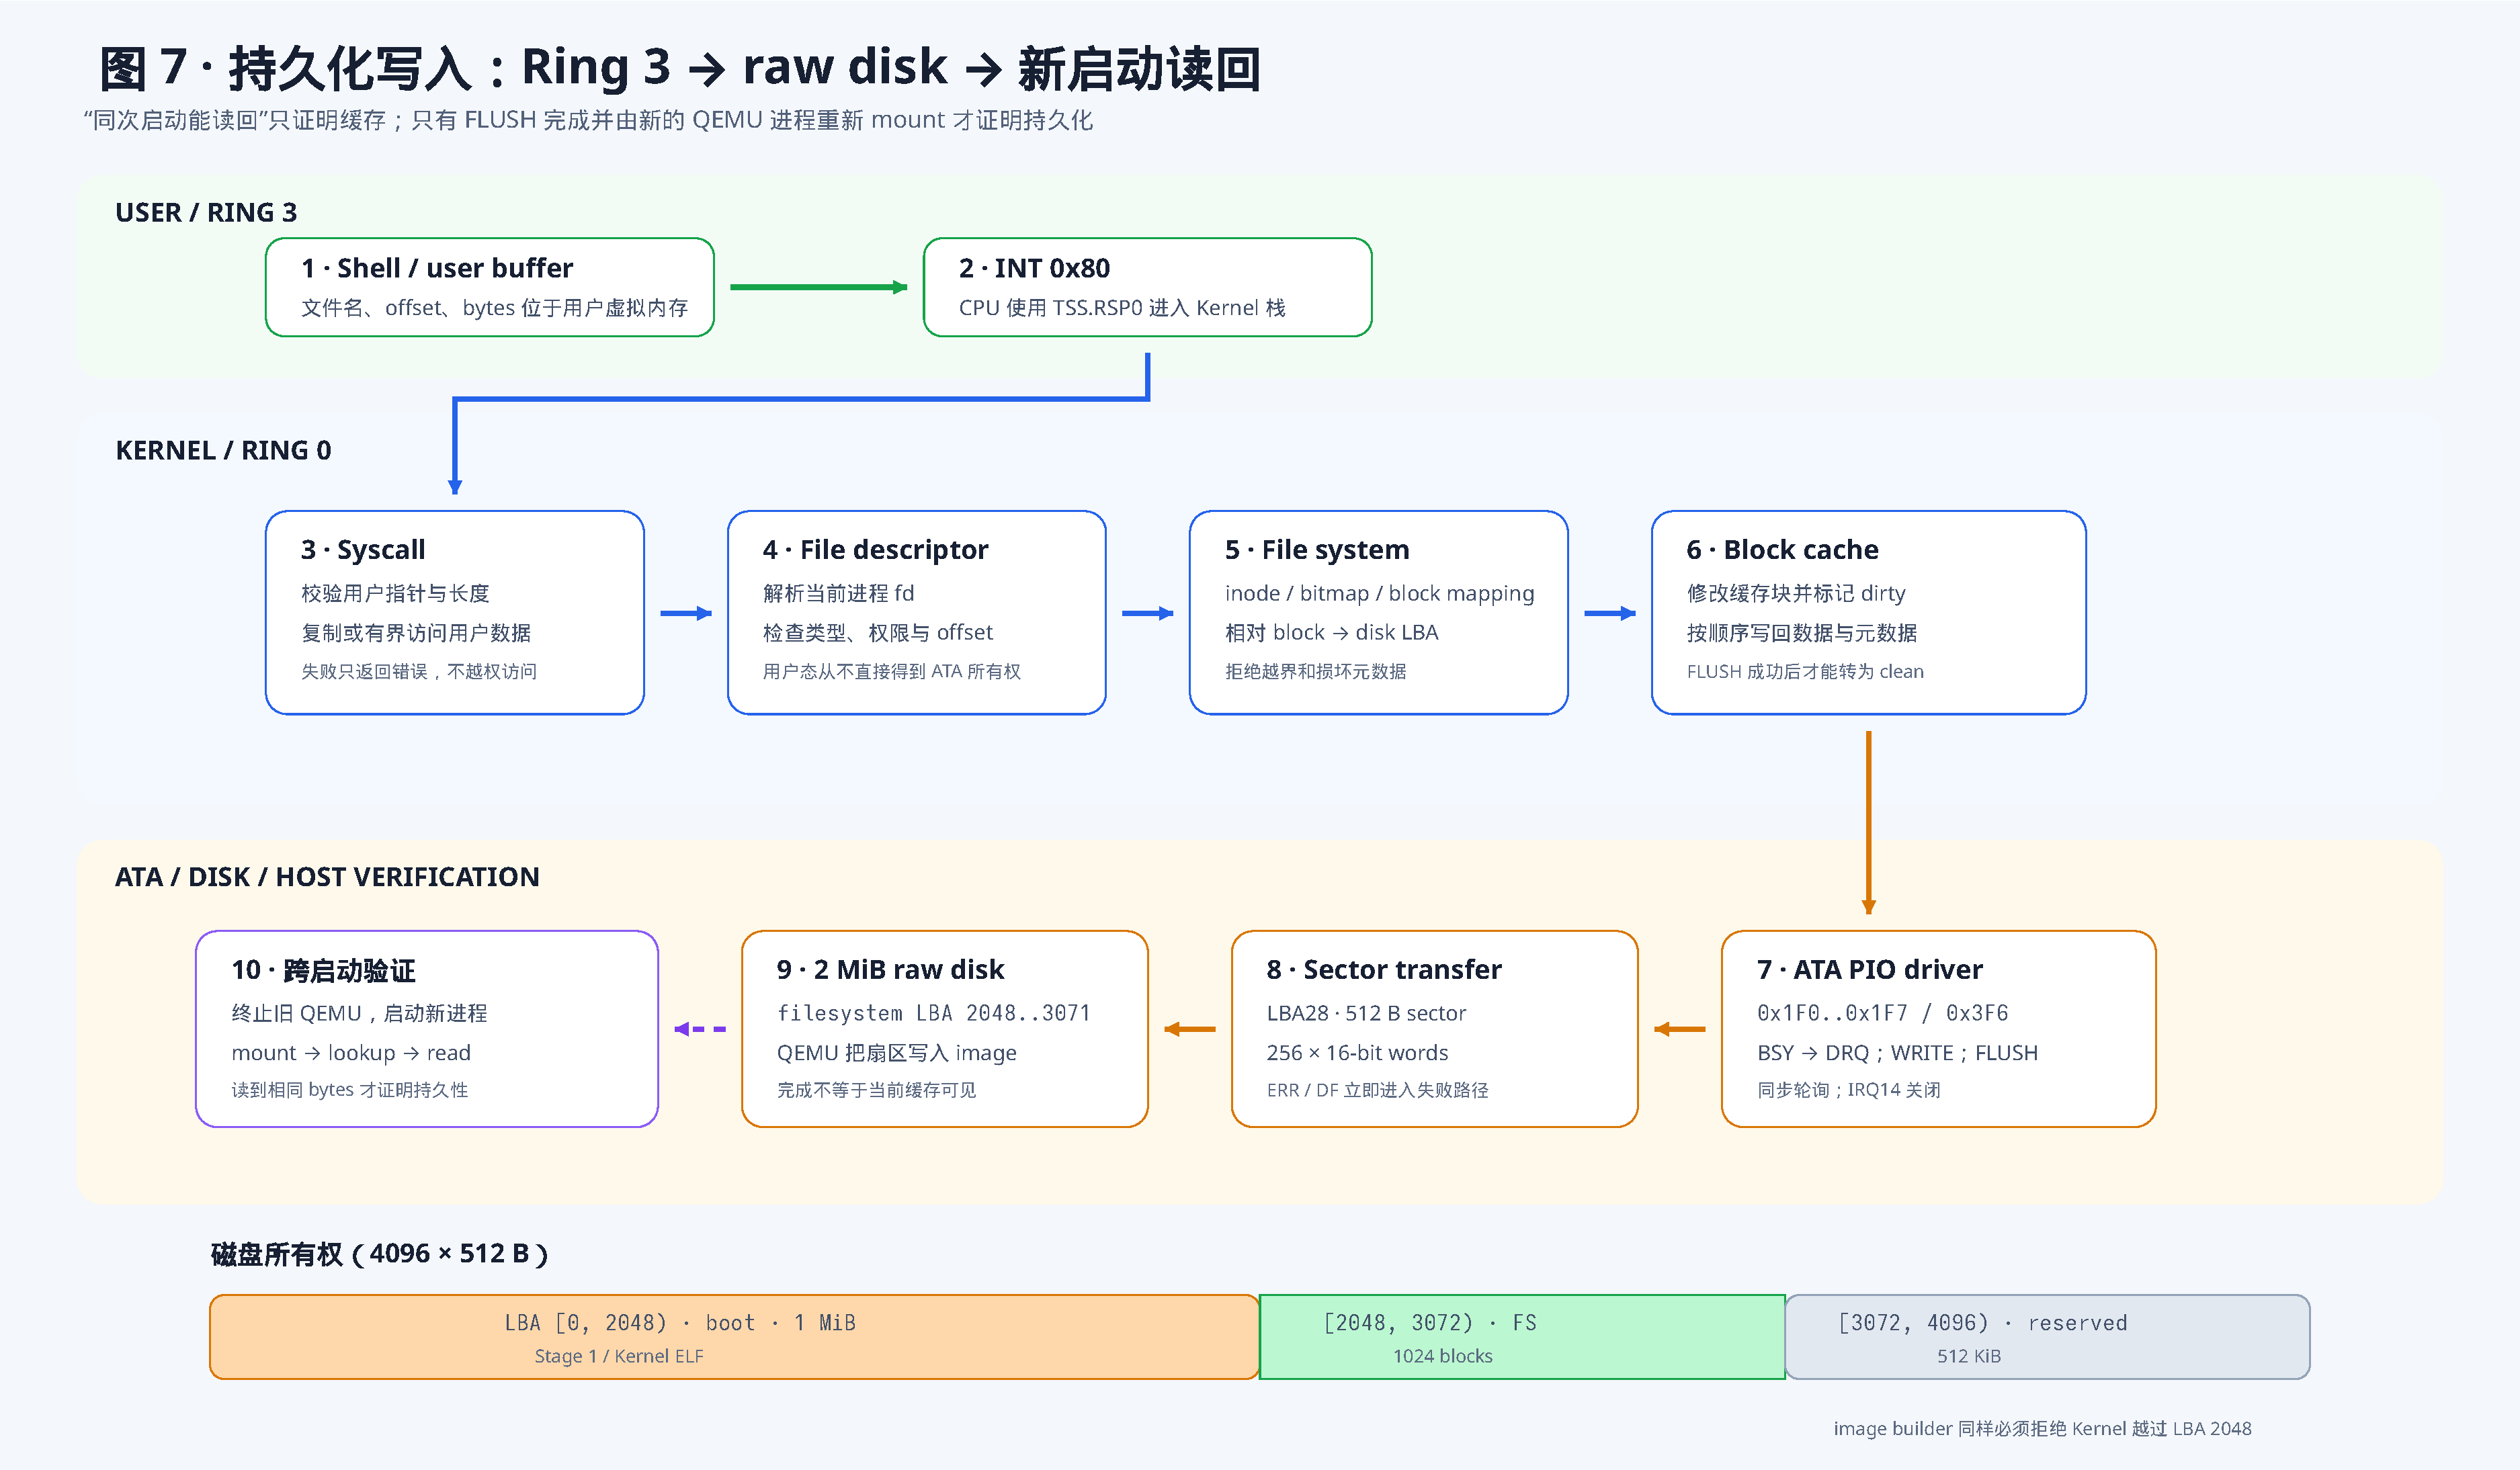
\includegraphics[width=0.96\textheight,height=0.82\textwidth,keepaspectratio]
    {figures/system_wiring/storage_persistence.pdf}
  \caption{Ring 3 文件写入到 raw disk、再由新 QEMU 启动读回的完整矢量路径。
  绿线表示用户请求，蓝线表示内核对象与数据流，橙线表示 ATA/磁盘传输，紫线
  表示跨进程验证；下方同时给出 4096 个扇区的磁盘所有权分区。}
  \label{fig:storage-persistence-full}
\end{sidewaysfigure}
\clearpage

\topic{一、先区分“可见”“已写回”和“持久”}\par
\begin{osgridlongtable}{L{0.20\linewidth}L{0.29\linewidth}L{0.31\linewidth}L{0.10\linewidth}}
结论 & 已经证明 & 还没有证明 & 强度 \\ \hline
write 返回成功 & 内核接受请求并按接口完成当前提交点 & 数据已离开全部 volatile cache & 低 \\ \hline
同次启动读回相同 & 当前内核路径能从缓存或磁盘返回字节 & 重启后仍存在 & 较低 \\ \hline
ATA WRITE 完成 & 控制器接受/处理数据传输 & 设备内部易失缓存已稳定落介质 & 中 \\ \hline
FLUSH 成功 & 设备按当前 ATA 协议完成缓存刷新 & 新启动的 mount/读取逻辑也正确 & 较高 \\ \hline
新 QEMU 进程读回 & 旧进程和所有 Guest RAM 已消失，镜像重新挂载后字节一致 & 任意断电点都有日志级原子恢复 & 当前最强 \\ \hline
\end{osgridlongtable}

\term{持久性}{persistence}表示状态在产生它的执行实例结束后仍可恢复；
\term{耐久性}{durability}通常强调已经承诺成功的数据在规定故障模型下不会
丢失。当前项目检查正常 FLUSH 后跨 QEMU 进程保存；写到任意中间位置突然
断电的恢复由后文 journal、写序和 replay 实验覆盖。

\topic{二、步骤 1--3：用户地址必须在边界上重新验证}
Shell 的文件名、offset 和 bytes 位于用户虚拟地址空间。用户程序执行
\code{INT 0x80} 后，CPU 按 IDT gate 与 TSS.RSP0 切入当前进程的 Ring 0 栈。
硬件只完成特权和栈转换，不会替 Kernel 判断指针安全。

系统调用层必须同时检查：

\begin{itemize}[leftmargin=2em]
  \item 系统调用号存在，参数个数和宽度符合 ABI；
  \item 用户地址处于允许范围，地址加长度不溢出；
  \item 每个跨页范围都具有用户访问和所需读/写权限；
  \item 字符串有最大长度和终止边界，不能无限扫描；
  \item 复制失败只返回确定错误，不把半写内核状态提交给下一层。
\end{itemize}

Kernel 不应在持有可能阻塞其他路径的锁时直接访问可故障用户页。当前模型虽比
完整 demand paging 简单，仍应维持“验证/复制用户数据”与“修改持久对象”的
清楚提交顺序。

\topic{三、步骤 4：fd 不是 inode，也不是磁盘地址}
\term{file descriptor}{文件描述符，fd}只是当前进程 FileTable 中的整数索引。
FileTable 项引用 KernelObject；文件类型进一步引用共享 FileDescription，
后者保存打开状态和当前 offset；文件系统对象再关联 inode。多层间接让复制 fd
可以共享 offset，而两次独立 open 可以得到不同 offset。

\[
\mathrm{fd}
\rightarrow \mathrm{FileTable\ entry}
\rightarrow \mathrm{KernelObject}
\rightarrow \mathrm{FileDescription}
\rightarrow \mathrm{inode/file}.
\]

每一箭头都带引用和权限语义。关闭 fd 只删除当前表项并释放相应引用；只有最后
引用离开时对象才析构。把 fd 数字直接当 inode 编号，会破坏跨进程共享、类型
检查和生命周期。

\topic{四、步骤 5：文件系统把名字和 offset 变成磁盘块}
\term{inode}{索引节点}保存文件类型、大小和数据块映射；
\term{bitmap}{位图}用 bit 记录 inode 或 block 是否已占用；
\term{directory entry}{目录项}把名称关联到 inode；
\term{superblock}{超级块}冻结磁盘格式、范围和校验。一次路径解析依次读取
目录项和 inode，文件 offset 再映射到相对 block，最后加上文件系统分区起点
得到全盘 LBA。

这些结构使用显式小端编码，不能把编译器内存中的 C++ struct 原样写盘。结构体
可能包含 padding、不同对齐或宿主字节序；磁盘格式必须对每个字段宽度、偏移、
合法范围和校验和负责。

\topic{五、步骤 6：block cache 为什么需要 dirty/clean 状态}
块缓存保留近期磁盘块的 RAM 副本，避免每次读写都发 ATA 命令。
\term{dirty}{脏}表示 RAM 副本比持久介质更新；
\term{clean}{干净}表示该副本与已确认的介质状态一致。把内存改完不应立即标
clean；只有数据、元数据按协议写出并完成必要 FLUSH，才能推进状态。

写回次序会影响故障后可解释性。若目录项先指向尚未写好的 inode，或 inode
先指向尚未分配/写好的数据块，断电后会出现悬空引用。当前固定布局使用明确的
Dirty/Clean 提交和全盘一致性检查；更完整的 v2 方案用 ordered metadata
journal 进一步定义崩溃恢复边界。

\topic{六、步骤 7--8：ATA PIO 把一个扇区变成 256 个 word}
驱动向 primary ATA 的任务文件寄存器写 LBA28、扇区数和命令，轮询 BSY、DRQ、
ERR 与 DF。数据口 \code{0x1F0} 按 16 位访问，一个 512 B 扇区需要传输
256 个 word。控制寄存器和状态寄存器仍按 8 位访问，不能为了循环方便把整组
端口都改成同一宽度。

\term{sector}{扇区}是当前 ATA 传输的 512 B 单位；
\term{LBA}{Logical Block Address}是扇区编号；
\term{filesystem block}{文件系统块}是文件系统分配和缓存单位。当前图中两者
同为 512 B，概念仍不能合并，因为未来文件系统可用多个 sector 组成一个 block，
NVMe 也有自己的 namespace 与 logical block 规格。

\topic{七、步骤 9：raw disk 是镜像容器，不等于文件系统}
\term{raw disk image}{原始磁盘镜像}按扇区保存整块虚拟磁盘，没有宿主文件系统
替 Guest 自动解释内容。v0.11 的历史 2 MiB 镜像共有
\[
4096\times512\ \mathrm{B}=2\ \mathrm{MiB}.
\]

\begin{osgridlongtable}{L{0.22\linewidth}L{0.22\linewidth}L{0.25\linewidth}L{0.21\linewidth}}
LBA 半开区间 & 大小 & 所有者 & 内容 \\ \hline
\([0,2048)\) & 1 MiB & 启动镜像布局 & Stage 1、Kernel 容器/ELF 与保留结构 \\ \hline
\([2048,3072)\) & 512 KiB & 文件系统 & 1024 个当前文件系统块 \\ \hline
\([3072,4096)\) & 512 KiB & 明确保留 & 不允许 Kernel 镜像或文件系统越界占用 \\ \hline
\end{osgridlongtable}

半开区间让长度等于 end-start，相邻区域可以无歧义拼接。镜像构建器和 Kernel
都必须拒绝越过边界；否则一次大文件写入可能覆盖下一次启动所需的 Kernel，
表面文件系统成功却让机器再也不能启动。

自 v1.6 起镜像已扩为逻辑 1 GiB 稀疏文件；v1.9 当前从 LBA 32768 起分配
固定 256 MiB rootfs。本表保留为第一版持久格式的历史基线，详细新布局见本章
后续 rootfs v2 节。

\topic{八、步骤 10：为什么必须终止旧 QEMU}
如果只在同一个 Guest 中 unmount/mount 或重新读取，RAM 中仍可能保留缓存、
对象和错误的未写回副本。自动测试先等待写入、sync 和成功标记，再终止旧 QEMU
进程；随后用同一磁盘文件启动全新的 QEMU。新 Guest 的 CPU、RAM、Kernel 堆和
块缓存均重新建立，只能从 disk image 读取状态。

新启动必须通过 superblock 验证、mount、路径查找、inode/block 读取，最终得到
精确相同字节。测试还要使用禁止标记确保没有悄悄格式化损坏磁盘、没有走错误
恢复分支，超时则视为失败而非“可能还在写”。

\topic{九、把 QEMU ATA 换成实体 NVMe 时哪些层保持}
文件描述符、FileDescription、路径、inode、bitmap、块缓存和大部分文件系统
规则可以保持；最下层块设备驱动和发现路径必须替换。DFR1142 的 M.2 M Key
连接 PCIe x1，常见 SSD 使用 NVMe，而当前 STUOS 只驱动 QEMU 的 legacy ATA
PIO。实体适配至少还需：

\begin{enumerate}[leftmargin=2.2em]
  \item 通过 UEFI/ACPI/PCIe 配置空间发现 root 与 NVMe function；
  \item 分配/读取 BAR，把控制器 MMIO 映射成正确缓存属性；
  \item 建立 admin/I/O submission 与 completion queue；
  \item 为队列和数据准备 DMA 可见物理内存，处理 doorbell 与完成中断/轮询；
  \item 把 NVMe namespace block 接到现有 BlockDevice 抽象，并重新验证
        FLUSH/持久性语义。
\end{enumerate}

所以“载板有 M.2”只证明物理插槽和 PCIe 通道存在；“Kernel 有文件系统”只证明
上层格式和对象模型存在。中间 PCIe/NVMe 驱动链没有实现时，两端不能自动接通。

\topic{十、失败现象怎样对应到十步链}\par
\begin{osgridlongtable}{L{0.25\linewidth}L{0.31\linewidth}L{0.34\linewidth}}
现象 & 最可能边界 & 应保存的证据 \\ \hline
write 立即返回参数错误 & 用户复制、fd 类型/权限或范围检查 & syscall 号、fd、长度、精确错误码 \\ \hline
同次读回正确、重启丢失 & dirty cache、ATA WRITE/FLUSH 或镜像绑定 & dirty/clean 计数、状态位、FLUSH 标记 \\ \hline
重启后自动格式化 & mount 的全零/损坏分类错误 & superblock 原始字节、CRC、禁止标记 \\ \hline
小文件正常、大文件破坏启动 & block/LBA 边界或长度溢出 & 目标半开区间、镜像审计、受影响 LBA \\ \hline
第二次 QEMU 读到旧内容 & 旧进程未终止、磁盘文件错误或 flush 未完成 & 进程边界、镜像路径/hash、完成标记 \\ \hline
随机卡在 ATA & BSY/DRQ/ERR/DF 轮询与预算 & 最后状态、命令、LBA、剩余 timeout \\ \hline
\end{osgridlongtable}

端到端测试证明整条链能协作，单元/随机测试则分别证明路径解析、位图、cache、
fd 和状态机边界。两者不能互相替代：只跑 QEMU 很难覆盖每个损坏字段，只跑
内存模型又不能证明真实 ATA 端口和跨启动镜像。

\input{deepening/ch13-irq14-writeback-v116}
\input{deepening/ch13-ordered-journal-v117}
